% Part   : Concepts
% Chapter: Corporate Identity
% ------------------------------------------------------------
% $Id: themes.tex 6207 2010-08-05 13:11:13Z al $
% ------------------------------------------------------------
\section{Themes}
\hypertarget{sec:Concepts:Identity:Themes}{}
\label{sec:Concepts:Identity:Themes}

\begin{description}
\item[framework:] trunk/Identity/Themes/
\end{description}

\noindent Here is where themes are produced.  In the above framework
location, themes are organized in ``Models'' ---to store common
information--- and ``Motifs''---to store unique information.  At
rendering time, both motifs and models are combined to produce the
final CentOS themes. CentOS themes can be tagged as ``default'' or
``alternative''. 

CentOS themes are maintained by CentOS community. 

% ------------------------------------------------------------
\section{CentOS Default Theme}
\hypertarget{sec:Concepts:Identity:Themes:Default}{}
\label{sec:Concepts:Identity:Themes:Default}

The CentOS default theme is used in all visual manifestations of
CentOS Project's corporate visual identity (e.g., distributions, web
sites, promotion, etc.).

Changing CentOS default theme is not very convenient because that
affects the ``recognition'' of CentOS Project.  Nevertheless, we are
interested on seeing your art work propositions.  Specially if your
art work is an improvement to the base idea behind CentOS default theme
(\textbf{Modern}, squares and circles flowing up.).

If you are not happy with CentOS default theme, you can look inside
CentOS alternative themes and download the one you are interested in.
If you are not happy with any of the CentOS alternative themes
available, then go and design your own CentOS alternative theme as
described in ``\hyperlink{sec:Concepts:Identity:Themes:Motifs}{Theme
Motifs}'' (\autoref{sec:Concepts:Identity:Themes:Motifs}).

% ------------------------------------------------------------
\section{CentOS Alternative Themes}
\hypertarget{sec:Concepts:Identity:Themes:Alternative}{}
\label{sec:Concepts:Identity:Themes:Alternative}

CentOS alternative themes exist for people how want to use a different
visual style on their installations of CentOS distribution. As the
visual style is needed for a system already installed components like
Anaconda are not required inside alternative themes. Inside
alternative themes you find post-installation visual style only (i.e.
Backgrounds, Display Managers, Grub, etc.).  CentOS alternative themes
are maintained by CentOS Community.

% ------------------------------------------------------------
\section{Theme Transition}
\hypertarget{sec:Concepts:Identity:Themes:Transition}{}
\label{sec:Concepts:Identity:Themes:Transition}

Theme transition is the action of moving a theme from alternative to
default.  This transition begins when an alternative theme gets
popular enough inside CentOS Comminity, and both CentOS Administrators
and CentOS Comunity Members want to extend it to all CentOS Visual
Manifestations. 

Once the popular alternative theme has been extended through all
CentOS visual manifestations, the alternative theme implementation
phase starts. The alternative theme implementation phase is where
default theme art work is replaced with alternative theme ones. After
the implementation phase, the previous default theme is tagged as
alternative and the implemented alternative as default.

Theme Transition has a huge impact in CentOS Corporate Visual
Identity, it should be done only if absolutly necessary. Generally, it
is better to improve the current default theme, based on its concept,
than create a completly new one. 

% ------------------------------------------------------------
\section{Theme Models}
\hypertarget{sec:Concepts:Identity:Themes:Models}{}
\label{sec:Concepts:Identity:Themes:Models}

\begin{description}
\item[framework:] trunk/Identity/Themes/Models/
\end{description}

\noindent Here is where theme models are stored.  Theme models let you
modeling characteristics (e.g., dimensions, translation markers,
position of each element on the display area, etc.) common to all
themes.  Theme models let you reduce the time needed when propagating
artistic motifs to different visual manifestations.

\begin{figure}[!hbp]
\hrulefill
\begin{verbatim}
trunk/Identity/Themes/
|-- Models
|   |-- Default             <-- theme's model name.
|   |   |-- Distro
|   |   |   |-- Anaconda
|   |   |   |   |-- Header
|   |   |   |   |-- Progress
|   |   |   |   |-- Prompt
|   |   |   |   `-- Splash
|   |   |   `-- BootUp
|   |   |       |-- Firstboot
|   |   |       |-- GDM
|   |   |       |-- GRUB
|   |   |       |-- GSplash
|   |   |       |-- KDM
|   |   |       |-- KSplash  
|   |   |       |-- RHGB
|   |   |       `-- Plymouth
|   |   |-- Promo
|   |   |-- Web
|   |-- Alternative        <-- theme's model name.
|   |   |-- Distro
|   |   |   `-- BootUp
|   |   |       |-- Firstboot
|   |   |       |-- GDM
|   |   |       |-- GRUB
|   |   |       |-- GSplash
|   |   |       |-- KDM
|   |   |       |-- KSplash  
|   |   |       |-- RHGB
|   |   |       `-- Plymouth
|   |-- ... more theme models.
\end{verbatim}
\hrulefill
\caption{Theme models structure.%
   \label{fig:Concepts:Identity:Themes:Models}}
\end{figure}

Theme models serves as a central pool of design templates for themes
to use. This way you can produce themes with different artistic motifs
but same characteristics.

Inside the framework location above, you find theme models organized
by name. You can add your own theme models to the structure by adding
a directory to the list. By default you have the following
ready-to-use theme models:

\begin{itemize}

\item \textbf{Default:} Stores the theme model used to produce
``\hyperlink{sec:Concepts:Identity:Themes:Default}{CentOS
Default Theme}''
(\autoref{sec:Concepts:Identity:Themes:Default}). 

\item \textbf{Alternative:} Stores the theme model used to produce
``\hyperlink{sec:Concepts:Identity:Themes:Alternative}{CentOS
Alternative Themes}''
(\autoref{sec:Concepts:Identity:Themes:Alternative}). 

\end{itemize}

\begin{figure}
\begin{center}
\fbox{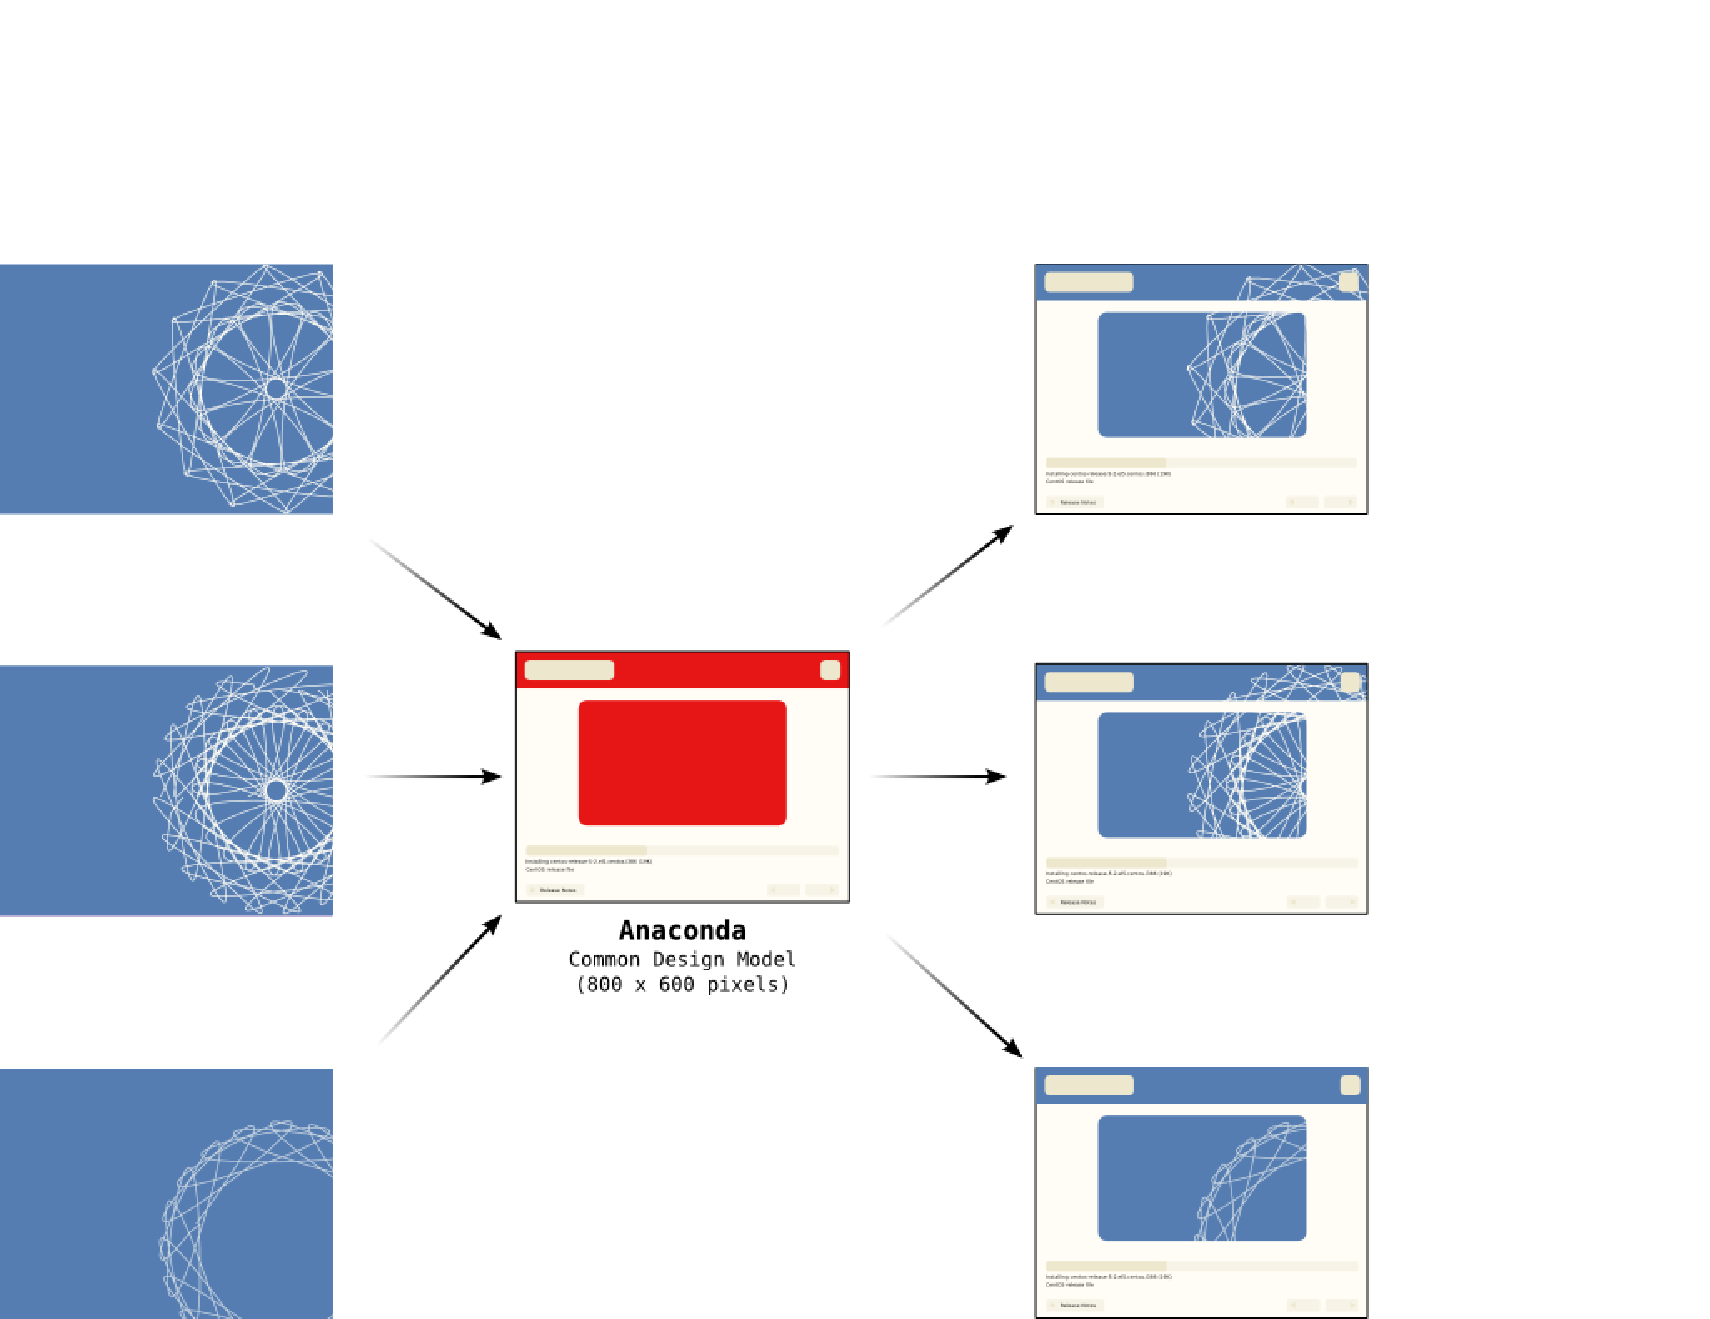
\includegraphics[width=0.8\textwidth]{%
   /home/centos/artwork/trunk/Identity/Models/Img/en/Corporate/common-design-model-fig1.pdf}}
\end{center}
\caption{Anaconda theme model producing three different visual
styles.}
\end{figure}

\begin{figure}
\begin{center}
\fbox{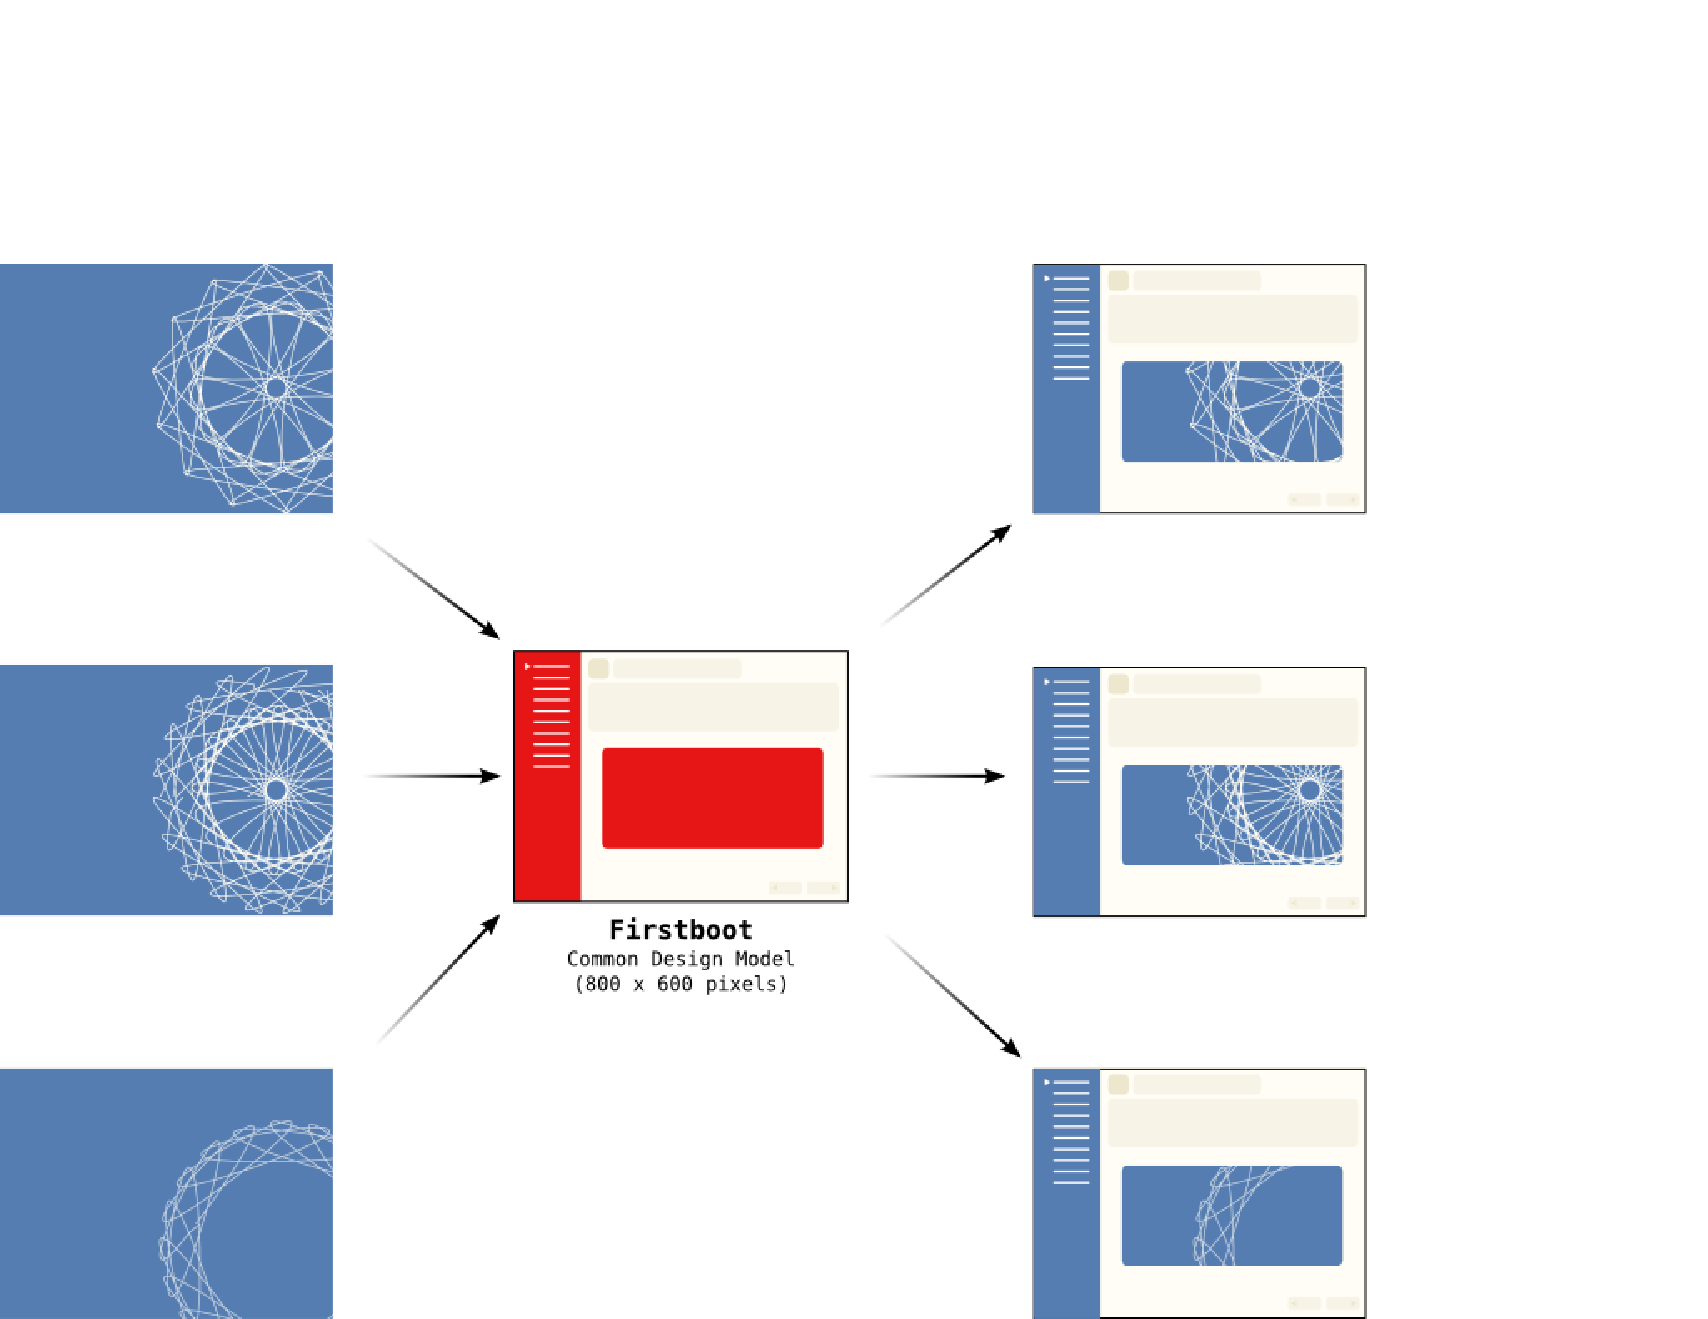
\includegraphics[width=0.8\textwidth]{%
   /home/centos/artwork/trunk/Identity/Models/Img/en/Corporate/common-design-model-fig2.pdf}}
\end{center}
\caption{Firstboot theme model producing three different visual
styles.}
\end{figure}

% ------------------------------------------------------------
\section{Theme Motifs}
\hypertarget{sec:Concepts:Identity:Themes:Motifs}{}
\label{sec:Concepts:Identity:Themes:Motifs}

\begin{description}
\item[framework:] trunk/Identity/Themes/Motifs/
\end{description}

\noindent Here is where the themes' artistic motifs are produced. The
artistic motif is a graphic design used as common pattern to connect
all CentOS Project's visual manifestations inside the same theme.

Inside the framework location above, artistic motifs are organized by
names inside the standard file structure illustrated in
\autoref{fig:Concepts:Identity:Themes:Motifs:Default} and
\autoref{fig:Concepts:Identity:Themes:Motifs:Alternative}.

\begin{figure}[!hbp]
\hrulefill
\begin{verbatim}
trunk/Identity/Themes/
|-- Motifs
|   |-- Modern              <-- theme name.
|   |   |-- Backgrounds
|   |   |-- Distro
|   |   |   |-- Anaconda
|   |   |   |   |-- Header
|   |   |   |   |-- Progress
|   |   |   |   |-- Prompt
|   |   |   |   `-- Splash
|   |   |   |-- BootUp
|   |   |   |   |-- Firstboot
|   |   |   |   |-- GDM
|   |   |   |   |-- GRUB
|   |   |   |   |-- GSplash
|   |   |   |   |-- KDM
|   |   |   |   |-- KSplash  
|   |   |   |   |-- RHGB
|   |   |   |   `-- Plymouth
|   |   |   `-- Desktop
|   |   |-- Info
|   |   |-- Palettes
|   |   |-- Promo
|   |   |-- Screenshots
|   |   `-- Web
|   |-- ... more theme names.
\end{verbatim}
\hrulefill
\caption{Theme motifs default structure.%
   \label{fig:Concepts:Identity:Themes:Motifs:Default}}
\end{figure}

\begin{figure}[!hbp]
\hrulefill
\begin{verbatim}
trunk/Identity/Themes/
|-- Motifs
|   |-- TreeFlower          <-- theme name.
|   |   |-- Backgrounds
|   |   |-- Distro
|   |   |   |-- BootUp
|   |   |   |   |-- Firstboot
|   |   |   |   |-- GDM
|   |   |   |   |-- GRUB
|   |   |   |   |-- GSplash
|   |   |   |   |-- KDM
|   |   |   |   |-- KSplash  
|   |   |   |   |-- RHGB
|   |   |   |   `-- Plymouth
|   |   |   `-- Desktop
|   |   |-- Info
|   |   |-- Palettes
|   |   |-- Screenshots
|   |-- ... more theme names.
\end{verbatim}
\hrulefill
\caption{Theme motifs alternative structure.%
   \label{fig:Concepts:Identity:Themes:Motifs:Alternative}}
\end{figure}

When designing artistic motifs for CentOS, consider the following
recommendations:

\begin{itemize}

\item Give a unique (case-sensitive) name to your Motif. This name is
used as value wherever theme variable (\$THEME) or translation marker
(\texttt{=THEME=}) is.  Optionally, you can add a description about
inspiration and concepts behind your work.

\item Use the location trunk/Identity/Themes/Motifs/\$THEME/ to store
your work. If it doesn't exist create it. Note that this require you
to have previous commit access in CentOS Artwork Repository.

\item The CentOS Project is using the blue color (\texttt{\#204c8d})
as base for its corporate visual identity. Use the CentOS Project's
base corporate color as much as possible in your artistic motif
designs.

\item Try to make your design fit one of the
``\hyperlink{sec:Concepts:Identity:Themes:Models}{Theme Models}''
(\autoref{sec:Concepts:Identity:Themes:Models}).

\item Feel free to make your art enterprise-level and beautiful.

\item Add the following information on your art work (both in a visible
design area, and inside Inkscape's document metadata section wherever
it be possible):

\begin{itemize}

\item The name (or logo) of your artistic motif.

\item The copyright sentence: \texttt{Copyright (C) YEAR YOURNAME}

\item The license under which the work is released. All CentOS Art
works are released under
\href{http://creativecommons.org/licenses/by-sa/3.0/}{Creative Common
Share-Alike License 3.0}
(\href{http://creativecommons.org/licenses/by-sa/3.0/}{http://creativecommons.org/licenses/by-sa/3.0/}).

\end{itemize}

\end{itemize}
% ------------------------------------------------------------
\section{Theme Palettes}
\hypertarget{sec:Concepts:Identity:Themes:Palettes}{}
\label{sec:Concepts:Identity:Themes:Palettes}

\begin{description}
\item[framework:] turnk/Identity/Themes/Motifs/\$THEME/Palettes/\\
\end{description}

\noindent Here is where graphic designers define theme palettes for
color-limited art works. Theme palettes contain the color information
that rendering functions need, in order to produce images with color
limitations.  Theme palettes contain theme's unique color information.
\autoref{tab:Concepts:Identity:Themes:Palettes:Files}.

% ------------------------------------------------------------
\section{Theme Palettes Creation}
\hypertarget{sec:Concepts:Identity:Themes:Palettes:Creation}{}
\label{sec:Concepts:Identity:Themes:Palettes:Creation}

Theme palettes are based on art works' specific color information you
are creating palettes for. As we write this section, there are two art
works that require color limitations. They are Grub and Syslinux art
works.

This section describes a generic procedure you can use to create theme
palettes for art works which need to be produced with color
limitations.

\begin{enumerate}

\item As first step, you need to produce a PNG file with the final
design of that art work you are creating palettes for.  You can do
this by using the \texttt{render.sh} script available in the art
work's identity framework.

\item Secondly, you need to generate the limited color information for
that PNG file the three different file formats (See
\autoref{tab:Concepts:Identity:Themes:Palettes:Files}). You can do
this by using the Gimp as described below: 

\begin{table}[!hbp]
\center
\begin{tabular}{ll}
\hline
\textbf{File} & \textbf{Description}\\
\hline
\texttt{.gpl} & Gimp palette files.\\
\texttt{.ppm} & Portable Pixel Map palette files.\\
\texttt{.hex} & Hexadecimal auxiliar palette files.\\
\hline
\end{tabular}
\caption{Palette file types.% 
   \label{tab:Concepts:Identity:Themes:Palettes:Files}}
\end{table}

\end{enumerate}

To create the \texttt{.gpl} file:

\begin{enumerate}

\item Open the Gimp (\textit{Applications / Graphics / The Gimp}).

\item Open the PNG format file you want to generate the limited color
information for (\textit{File / Open ...}).

\item Index the image (\textit{Image / Mode / Indexed...}).  This will
open the window ``Indexed Color Conversion''. Use this window to
``Generate optimum palette'' by setting the maximum number of colors
you want to have in the final indexed image. In this window, by the
default, Gimp has set 255 as the maximum number of colors, you should
change this value to fit the art work color limitation requirements
(i.e. 14 colors for Grub's splash, and 16 colors for Syslinux splash,
etc.). Another option you can play with is ``Color dithering'' at the
window's bottom, particularly the ``Floyd-Steinberg (reduced color
dithering)'' option which seems to archive the best results.

\item At this point you have reduced color information and indexed the
image. This let you save the color information as a Gimp palette file
(.gpl) for further using. 

To export the color information as Gimp palette you need to open the
palette window (\textit{Ctrl+P}) and go to the action ``Import
Palette...'' inside ``Palettes Menu''. This will open the window
``Import Palette''. In this window you need to specify the source from
where you will retrive color information and the name of the palette
file. Use ``Image'' as source to create your palette and the
appropriate name (e.g., \texttt{centos-\$themename-grub}).\footnote{in
\texttt{centos-\$themename-grub} file name, the \texttt{\$themename}
part is the theme's name you are working on (e.g., Modern, TreeFlower,
etc.) for Grub's palette, \texttt{centos-\$themename-syslinux} for
Syslinux palette, etc.}

\end{enumerate}

To create the \texttt{.ppm} file:

\begin{enumerate}

\item Use the Gimp to create a new image (\textit{Ctrl+N}) of 16 x 1
pixels of dimension.  That is 16 pixels width and 1 pixel height.
      
\item That is a rather small image so you problably want to zoom it in
to better see what you are doing. In a 1024x768 screen resolution,
zoom the 16 x 1 pixel image to 4500\% makes things clear enough. If
you are using a different screen resolution you probably need to zoom
in to a different value. 

\item Now it's time to fill up the empty image with the color
information we created previously. You do this using the pen tool
(\textit{N}) with a 1x1 brush (\textit{Shit+Ctrl+B}). At this point it
is a good time to open the ``Palette Editor'' window and use the Gimp
palette file with the color information we created (\textit{Ctrl+P /
doble click on the palette file}).

\begin{quote} 

\textbf{Caution!:} If you are creating \texttt{.ppm} palettes for
Anaconda prompt (syslinux), the order used to set the color
information is relevant. Relevant values in the image are positions: 0
and 7.  Position 0 is used as background color, which is black
(\texttt{\#000000}) generally and position 7 is used as forground
color, which is white (\texttt{\#ffffff}) generally. This, in order to
grant the highest contrast.  See
\autoref{fig:Concepts:Identity:Themes:Palettes:Syslinux}.

\end{quote}
      
\end{enumerate}

To create the (\texttt{.hex}) file:

\begin{enumerate}

\item Create a plain text file and put the hexadecimal color
information and its index position defined in \texttt{.ppm} palette
inside the file, one definition by line.  The format used to create
the \texttt{.hex} file is \texttt{\#rrbbgg=i \dots}.  Where
\texttt{\#rrggbb=i} indicates that the color \texttt{\#rrggbb} (hex)
should be assigned index i (decimal).

\begin{quote}
\textbf{Caution!:} In order to produce Anaconda prompt (syslinux)
images correctly, both \texttt{.hex} and \texttt{.ppm} color and index
information should match.
\end{quote}

\end{enumerate}

\begin{figure}[!hbp]
\begin{center}
\fbox{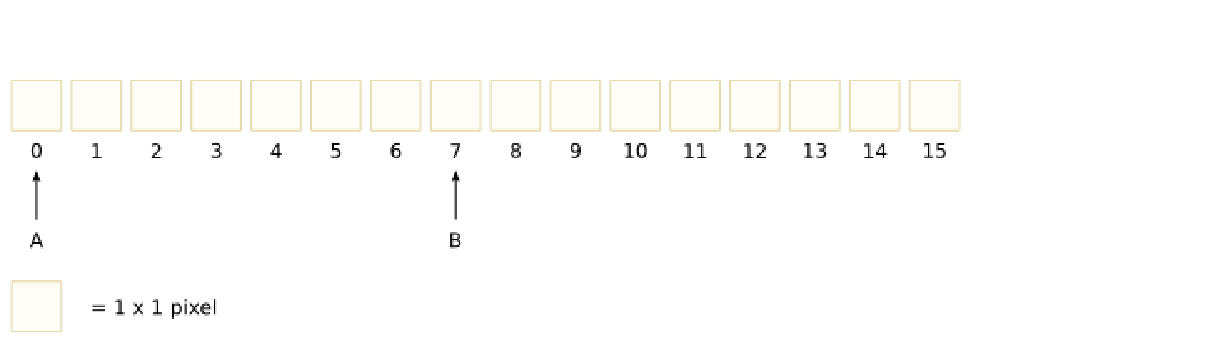
\includegraphics[width=0.8\textwidth]{%
   /home/centos/artwork/trunk/Identity/Models/Img/en/Distro/Anaconda/Prompt/syslinux-palette.pdf}}
\end{center}
\caption{Palette's background (A) and forground (B) color position.%
    \label{fig:Concepts:Identity:Themes:Palettes:Syslinux}}
\end{figure}

% ------------------------------------------------------------
\section{Theme File Structure}
\hypertarget{sec:Concepts:Identity:Themes:Files}{}
\label{sec:Concepts:Identity:Themes:Files}

Inside CentOS Artwork Repository, each theme has a name and a
directory for it. Inside each theme directory, the CentOS Project
visual style is organized in the directories: Distro, Info, Palettes,
Promo, Screenshots, and Web. 

% ------------------------------------------------------------
\subsection{The \texttt{Distro} Directory}
\hypertarget{sec:Concepts:Identity:Themes:Files:Distro}{}
\label{sec:Concepts:Identity:Themes:Files:Distro}

Here is where image files controlling CentOS Distribution visual style
are produced. 

\begin{figure}[!hbp]
\hrulefill
\begin{verbatim}
turnk/Identity/Themes/Motifs/$THEME/Distro/
|-- Anaconda
|   |-- Header
|   |-- Progress
|   |-- Prompt
|   `-- Splash
|-- BootUp
|   |-- Firstboot
|   |-- GDM
|   |-- GRUB
|   |-- GSplash
|   |-- KDM
|   |-- KSplash
|   `-- RHGB
`-- Desktop
\end{verbatim}
\hrulefill
\caption{The CentOS distribution theme structure.}
\end{figure}

% ------------------------------------------------------------
\subsection{The \texttt{Palettes} Directory}
\hypertarget{sec:Concepts:Identity:Themes:Files:Palettes}{}
\label{sec:Concepts:Identity:Themes:Files:Palettes}

Here is where theme's palettes are sotred. Palettes are used to
automate image rendering in cases where a limited amount of color need
to be specified. Before you could render color-limited art works (e.g.
Grub, and Syslinux), you need to create their color-limited palettes
first. See
``\hyperlink{sec:Concepts:Identity:Themes:Palettes:Creation}{Theme
Palette Creation}''
(\autoref{sec:Concepts:Identity:Themes:Palettes:Creation}).

% ------------------------------------------------------------
\subsection{The \texttt{Promo} Directory}
\hypertarget{sec:Concepts:Identity:Themes:Files:Promo}{}
\label{sec:Concepts:Identity:Themes:Files:Promo}

Here is where image files controlling CentOS promotion visual style
are produced.

% ------------------------------------------------------------
\subsection{The \texttt{Screenshots} Directory}
\hypertarget{sec:Concepts:Identity:Themes:Files:Screenshots}{}
\label{sec:Concepts:Identity:Themes:Files:Screenshots}

Here is where theme's screenshots are stored. The purpose of this
directory is to collect theme's implementation graphical history
through time. Inside this directory you can have distribution
screenshots, web sites screenshtos, and promotion screenshots. If
theme has been implemented out of computers like would be the case of
events, stands, etc. those photos can be added here too, in the
promotion screenshot section.

% ------------------------------------------------------------
\subsection{The \texttt{Web} Directory}
\hypertarget{sec:Concepts:Identity:Themes:Files:Web}{}
\label{sec:Concepts:Identity:Themes:Files:Web}

Here is where image files controlling CentOS Web sites visual style
are produced.
